\documentclass[a4paper,12pt]{article}
\usepackage{graphicx}
\usepackage{amsmath}
\usepackage{float}
\usepackage{hyperref}
\usepackage{geometry}
\usepackage{listings}
\usepackage{xcolor}
\geometry{top=1in, bottom=1in, left=1in, right=1in}

% Define colors for a fresh, readable style
\definecolor{keywordcolor}{RGB}{0, 102, 204}   % Keywords (blue)
\definecolor{stringcolor}{RGB}{183, 28, 28}    % Strings (red)
\definecolor{commentcolor}{RGB}{85, 107, 47}  % Comments (green)
\definecolor{bgcolor}{RGB}{245, 245, 245}      % Light gray background
\definecolor{numbercolor}{RGB}{150, 150, 150}  % Line numbers

% Configuration for code listings
\lstset{
    backgroundcolor=\color{bgcolor},     % Background color
    basicstyle=\ttfamily\footnotesize,   % Code font and size
    keywordstyle=\color{keywordcolor}\bfseries, % Bold keywords
    stringstyle=\color{stringcolor},     % String color
    commentstyle=\color{commentcolor}\itshape, % Italic comments
    numberstyle=\color{numbercolor}\tiny, % Line numbers
    numbers=left,                        
    stepnumber=1,                        
    breaklines=true,                     
    showstringspaces=false,              
    frame=single,                        
    rulecolor=\color{gray},              % Frame color
    tabsize=4,
    captionpos=b,                        
    xleftmargin=1em,
    framexleftmargin=0em,
}

\title{Implementation and Performance Analysis of Bitonic Sort using CUDA}

\author{
    \small Aristotle University of Thessaloniki - Department of Electrical and Computer Engineering \\[0.5em]
    \small Parallel and Distributed Systems\\[1.5em]
    Koumparidou Eleni and Maria Sotiria Kostomanolaki \\[1em]
}
\date{January 2025}

\begin{document}

\maketitle

\begin{abstract}
This project implements a parallel sorting algorithm using \textbf{CUDA}, based on the Bitonic Sort algorithm. The goal is to explore different strategies for parallelizing the Bitonic Sort algorithm using CUDA. The program sorts $N = 2^q$ integers in ascending order, leveraging GPU parallelism to accelerate the sorting process. Three versions of the algorithm have been developed (V0, V1, V2), each one using a different aspect of parallelism (thread-level parallelism, kernel synchronization, shared memory usage).. Each implementation aims to improve the usage of CUDA's resources using different CUDA features to achieve high-performance and higher speed sorting. The correctness and the execution time of this algorithm for different input sizes ($q \in [20, 27]$) are compared to the quickSort (\texttt{qSort}) algorithm, implemented in C. Performance tests on the Aristotelis cluster highlight the speedup achieved by GPU parallellism and demonstrate the impact of CUDA on sorting efficiency.
\end{abstract}

\tableofcontents
\newpage

\section{Introduction}
Before presenting the implementation, we provide an overview of the Bitonic Sort algorithm and the optimization approaches explored in this assignment. Three progressively improved versions of the algorithm are introduced, each leveraging CUDA's capabilities to enhance sorting performance.


\subsection{Background: Bitonic Sort Algorithm}  
\textbf{Bitonic Sort} is a sorting algorithm that recursively transforms an unsorted sequence into a bitonic sequence. A \textbf{bitonic sequence} is a sequence of numbers that first monotonically increases and then monotonically decreases (or vice versa). It consists of two main steps: 
\begin{enumerate}
 \item \textbf{Bitonic Merge:} This step takes a bitonic sequence and produces a fully sorted sequence by separating the elements into two subsequences containing minima and maxima, based on elementwise comparisons. The process is recursively repeated for each half. The time complexity of Bitonic Merge is \(O(n \log n)\).  

\item \textbf{Bitonic Sort:} This recursively divides the input sequence, sorting one half in ascending order and the other in descending order to form a bitonic sequence. Bitonic Merge is then applied to produce the final sorted result. The overall time complexity of Bitonic Sort is \(O(n (\log n)^2)\).  
\end{enumerate}
For the C implementation of the serial algorithm and a visualization, you can refer to the following excellent resource \cite{sortvisualizer}.

\subsubsection*{Key Terms}
The following key terms will be used throughout the report:
\begin{itemize}
    \item \textbf{\texttt{group\_size}}: It represents the amount of elements from the array that will follow the same sorting pattern for each pass of the Bitonic Sort algorithm. Initially set to 2, the \texttt{group\_size} doubles with each iteration until the whole array is sorted.
    \item \textbf{\texttt{distance}}: The gap between elements that need to be compared during each sorting step. In every sorting phase of the algorithm distance is taking the following values:
    \[
    \left[ \frac{\text{group\_size}}{2}, \dots, 2, 1 \right]
    \]
    \item \textbf{partner}: The element that needs to be compared with the chosen element. 
    \item \textbf{threads}: Individual units within a CUDA block. Threads work in parallel to process elements in the array.
    \item \textbf{blocks}: Groups of threads in CUDA. A block can hold up to 1024 threads, and the threads within a block cooperate to perform part of the sorting task.
\end{itemize}

\subsection{CUDA Memory Model Overview}
Each Version is based on a different type of CUDA memory in order to reduce latency. We will use the following, that can be seen also as a diagram in \ref{fig:CUDA}.

\begin{itemize}
    \item \textbf{Global Memory}: Every grid, block or thread have access to it.
    \item \textbf{Local Memory}: The threads within the same block share the local memory.
    \item \textbf{Shared Memory}: The threads within the same block have access to shared memory. It has smaller latency than other two memories.

    
\end{itemize}


\begin{figure}[H]
    \centering
    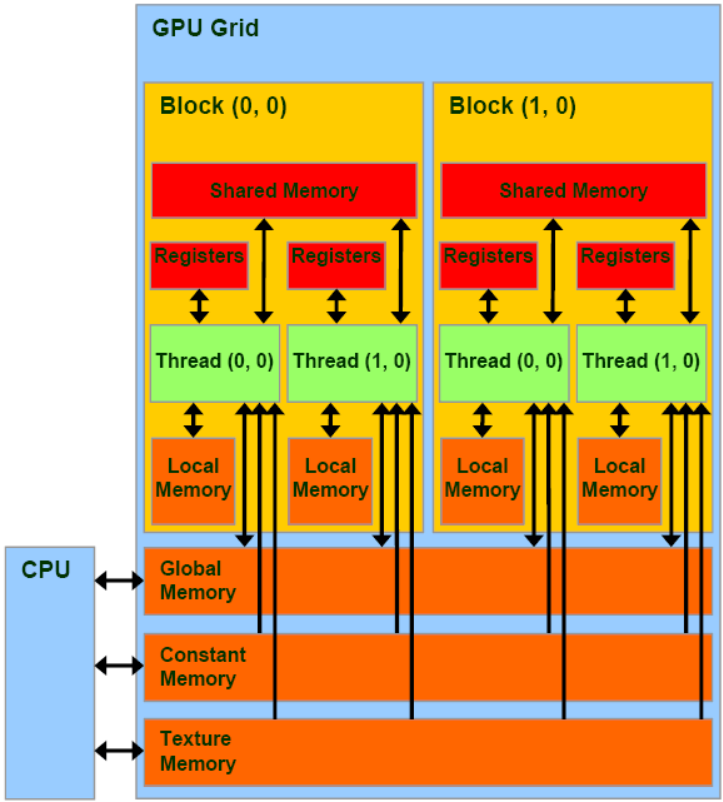
\includegraphics[width=0.5\linewidth]{assets/CUDA Memory Model.png}
    \caption{CUDA Memory Model}
    \label{fig:CUDA}
\end{figure}






\section{Algorithm Description}

The main function of the implementation starts by allocating memory on both the CPU and GPU for an array of size \(2^q\), where \(q\) is specified by the user at the \texttt{make run} command and ranges from 20 to 27. This dual memory allocation is essential because the CPU and GPU have separate memory spaces. A CPU (host) function can only access CPU memory, while GPU functions (kernels) can only access GPU memory. Therefore, two separate arrays are required: one on the CPU and one on the GPU. 

After memory allocation, the CPU array is initialized with random integers, and the data is copied to the GPU. The function \texttt{bitonicSort()} is then called to sort the elements. The implementation of this function varies depending on the selected version (V0, V1, or V2). 

Once the sorting operation is completed, the results are copied back to the CPU. Finally, the program evaluates the correctness of the sorting operation and calculates the execution time.

The following subsections describe the differences between each version of the algorithm and the CUDA features utilized.

\subsection{V0: Basic Parallel Implementation}

Version 0 implements the Bitonic Sort algorithm using the fundamentals of parallel programming in CUDA. This version introduces a straightforward approach to parallel sorting using GPU threads.
The main idea is to assign in each thread the task of \textbf{comparing} and potentially swapping two elements in the array. This is done using the \texttt{exchange\_V0} kernel function in Listing \ref{lst:exchangeV0}.
\\
\begin{lstlisting}[language=C, caption={Exchange process using GPU's threads}, label={lst:exchangeV0}]
    __global__ void exchange_V0(int *array, int size, int group_size, int distance) {
    int tid = threadIdx.x + blockIdx.x * blockDim.x;
    int idx = (tid / distance) * distance * 2 + (tid % distance);
    int partner = idx ^ distance;
    bool sort_descending = idx & group_size;

    if (idx < size && partner < size && idx < partner){ 
        if (!sort_descending && array[idx] > array[partner]){
            swap(array, idx, partner);  // keep min elements   }
        if (sort_descending && array[idx] < array[partner]) {
            swap(array, idx, partner);   // keep max elements  }
    }
}
\end{lstlisting}
To call the previous kernel we use the maximum number of threads, 1024, and the blocks that are needed to manage all the elements of the array. These parameters are definied in \texttt{bitonicSort} function in Listing \ref{lst:bitonicV0}.
\\
\begin{lstlisting}[language=C, caption={Kernel call for elementwise comparison using threads}, label={lst:bitonicV0}]
void bitonicSort(int *array, int size)
{
    // GPU PARAMETERS
    int threads_per_block = 1024;  
    int blocks_per_grid = size / threads_per_block; 

    for (int group_size = 2; group_size <= size; group_size <<= 1){ 
        for (int distance = group_size >> 1; distance > 0; distance >>= 1)
            exchange_V0<<<blocks_per_grid, threads_per_block>>>(array, size, group_size, distance);}
    }
\end{lstlisting}

 



\subsubsection*{Index Calculation}

A critical aspect of this approach is to assign elements to threads by calculating the array index (\texttt{idx}) as a function of the current thread ID (\texttt{tid}). This management is not handled by CUDA, so it is calculated by the following expression:
\\
\begin{lstlisting}[language=C]
int idx = (tid / distance) * distance * 2 + (tid % distance);
\end{lstlisting}

Here is a breakdown of the formula:
\begin{itemize}
    \item \texttt{(tid / distance)}: Computes which block the thread belongs to for this particular step of the sorting process.
    \item \texttt{* distance * 2}: Takes into consideration the fact that comparisons are made between pairs separated by twice the \texttt{distance}.
    \item \texttt{(tid \% distance)}: Identifies the thread’s relative position within its block.
\end{itemize}

This formula guarantees a unique index for each thread, ensuring that every element in the array is correctly mapped for comparison during each stage of the Bitonic Merge process.

\subsubsection*{Swapping Elements on the GPU}

The swap of two elements is an important and often part of sorting. On the GPU, swaps are performed using the following device function:
\\
\begin{lstlisting}[language=C]
__device__ void swap(int *array, int idx, int partner) {
    int temp;
    temp = array[idx];
    array[idx] = array[partner];
    array[partner] = temp;
}
\end{lstlisting}


\subsubsection*{Synchronization Overhead}

In this version, every kernel call requires global synchronization across the GPU, which can be really "expensive" in terms of time. The processing must wait for all threads to finish their comparisons and swaps before proceeding to the next distance in the sorting step. The improvement of this delay is the goal for the next version (V1), which addresses this with the use of local block synchronization.

\subsection{V1: Local Block Synchronization}

Version V1 aims to improve the execution time of the algorithm developed in Version 0 by reducing the global synchronization cost. To achieve this, we take advantage of the local block synchronization, in which the threads inside the same block can be synchronized at a lower cost. 

The main idea is that, when the size of the array fits inside only one block, we call another kernel (\texttt{exchange\_V1}) that can make the whole exchange for all the distances for a specific group\_size at once. That means that if we have an array with 2048 elements, which needs 1024 comparisons in every stage of the sorting, it will be sorted with only one call.

\subsubsection*{Sorting Overview}
In order to use the property mentioned before, we rearrange the initial code (V0) using three kernels for the sorting process as is shown in Listing \ref{lst:bitSort1}:

\begin{itemize}
    \item \textbf{Initial sorting}: We make the exchanges for all groups of size less than 2048 using \texttt{initialExchange}. 
    \item \textbf{Exchanges for greater distances than 1024}: After the initial sorting when the distance is greater than 1024 we use \texttt{exchange\_V0} kernel (implemented in Version 0).
    \item \textbf{Exchanges for smaller distances than 1024}:
    After the initial sorting when the distance is smaller than 1024 or equal to we use \texttt{exchange\_V1} kernel.
    
\end{itemize}

\begin{lstlisting}[caption={Bitonic Sort algorithm of V1}, label={lst:bitSort1}]
    __host__ void bitonicSort(int *array, int size)
{
    // GPU PARAMETERS
    int threads_per_block = 1024;
    int blocks_per_grid = size / threads_per_block;

    initialExchange<<<blocks_per_grid, threads_per_block>>>(array, size);

    for (int group_size = 4096; group_size <= size; group_size <<= 1)
    { // group_size doubles in each reccursion

        for( int distance = group_size >> 1; distance > 1024; distance >>=1)
        {
            // Handle large distances (>1024)
            exchange_V0<<<blocks_per_grid, threads_per_block>>>(array, size, group_size, distance);
        }

        // Handle small distances (<=1024)
        exchange_V1<<<blocks_per_grid, threads_per_block>>>(array, size, group_size);
    }
}
\end{lstlisting}

\subsubsection*{Initial Exchange}
As we mentioned before the sorting algorithm starts by sorting small group sizes and doubles the \texttt{group\_size} until it reaches the full size of the array. This means that we can sort all groups until the group consists of 2048 elements. This reaches the limit of local block synchronization because the distance will start decreasing from distance of 1024, requiring 1024 exchanges for every distance, which can be managed by 1024 threads within a block. In the next recursion the distance will start from 2048, which requires 2048 threads for the exchange process divided into two blocks, that can be synchronized only from the global memory.

At the first part of this sorting we make the exchanges for all group sizes until 2048 using \texttt{initialExchange} function presented in Listing \ref{lst:initExchange}. This requires only one call of \texttt{initialExchange} in \texttt{bitonicSort}. After every exchange we call \texttt{\_\_syncthreads} function, so that all the threads within a block are up to date.
\\
\begin{lstlisting}[ caption={Initial Exchange}, label={lst:initExchange}]
__global__ void initialExchange(int *array, int size)
{
    int tid = threadIdx.x + blockIdx.x * blockDim.x;

    for (int group_size = 2; group_size <= 2048; group_size <<= 1)
    {
        for (int distance = group_size >> 1; distance > 0; distance >>= 1)
        {
            int idx = (tid / distance) * distance * 2 + (tid % distance);
            int partner = idx ^ distance;
            bool sort_descending = idx & group_size;

            if (idx < size && partner < size && idx < partner)
            { // ensure bounds are checked before accessing array

                if (!sort_descending && array[idx] > array[partner])
                {
                    // keep min elements
                    swap(array, idx, partner);
                }
                if (sort_descending && array[idx] < array[partner])
                {
                    // keep max elements
                    swap(array, idx, partner);
                }

                __syncthreads();
            }
        }
    }
}
\end{lstlisting}

\subsubsection*{V1 Exchange}
The only difference between the V0 and the V1 exchange is that there is a \texttt{for} loop inside the kernel so that all the exchanges until distance of 1024 happen at one kernel call, as it is shown in Listing \ref{lst:V1_ex}. A \texttt{\_\_syncthreads} call is again necessary after every exchange to ensure that all threads are updated.
\\
\begin{lstlisting}[caption={V1 Exchange algorithm}, label={lst:V1_ex}]  
__global__ void exchange_V1(int *array, int size, int group_size)
{
    int tid = threadIdx.x + blockIdx.x * blockDim.x;

    for (int distance = 1024; distance > 0; distance >>= 1)
    {
        int idx = (tid / distance) * distance * 2 + (tid % distance);
        int partner = idx ^ distance;
        bool sort_descending = idx & group_size;

        if (idx < size && partner < size && idx < partner)
        { // ensure bounds are checked before accessing array

            if (!sort_descending && array[idx] > array[partner])
            {
                // keep min elements
                swap(array, idx, partner);
            }
            if (sort_descending && array[idx] < array[partner])
            {
                // keep max elements
                swap(array, idx, partner);
            }

            __syncthreads();
        }
    }
}
\end{lstlisting}

\subsection{V2: Shared Memory Optimization}
V1 Version has already significant improvement in comparison to V0. The goal of V2 Version is to improve the performance of our algorithm even more using the shared memory provided by CUDA.

\subsubsection*{Shared Memory}
Shared memory is a memory provided by CUDA available for all threads within a block. The difference between shared memory and global or local memory is that threads have much easier and quicker access to shared memory. In fact, shared memory latency is roughly 100x lower than uncached global memory latency when no bank conflicts occur. 

\subsubsection*{Initial and V2 Exchange}
To use shared memory feature we adjust \texttt{initialExchange} and \texttt{exchange\_V1} kernel. To access an array through shared memory, we have to make a copy of the array from global memory to shared memory. We use three variables to handle the access of data:

\begin{itemize}
    \item \textbf{Local Thread Id}: The Id of a thread in shared memory.
    \item \textbf{Global Thread Id}: The position of an element in the global array.
    \item \textbf{Offset}: The distance from the first chunk of 2048 elements in the shared memory.
\end{itemize}

\begin{lstlisting}
    int local_tid = threadIdx.x;
    int global_tid = local_tid + blockIdx.x * blockDim.x;
    int offset = blockIdx.x * blockDim.x * 2;
\end{lstlisting}

We use the following two functions to load the array in shared memory and vice versa.
\begin{lstlisting}
__device__ void load_global_to_local(int *array, int *local_array, int size, int local_tid, int offset)
{
    if (local_tid + offset < size && local_tid + offset + blockDim.x < size)
    {
        local_array[local_tid] = array[local_tid + offset];
        local_array[local_tid + blockDim.x] = array[local_tid + offset + blockDim.x];

        __syncthreads();
    }
}

__device__ void load_local_to_global(int *array, int *local_array, int size, int local_tid, int offset)
{
    if (local_tid + offset < size && local_tid + offset + blockDim.x < size)
    {
        array[local_tid + offset] = local_array[local_tid];
        array[local_tid + offset + blockDim.x] = local_array[local_tid + blockDim.x];

        __syncthreads();
    }
}
\end{lstlisting}

We adjust \texttt{initialExchange} of V1 Version algorithm, so that we determine the index of the local array in shared memory using the parameters explained before.
\\
\begin{lstlisting}
    int global_idx = (global_tid / distance) * distance * 2 + (global_tid % distance);
    int idx = (local_tid / distance) * distance * 2 + (local_tid % distance);
    int partner = idx ^ distance;
    bool sort_descending = global_idx & group_size;
\end{lstlisting}
The same strategy is followed in \texttt{exchange\_V2} to load the array in shared memory and to access the right elements determined by the Bitonic Sort algorithm.

\section{Performance Analysis}
We tested every version (V1, V2, V3) in Aristotle Cluster, specifically in gpu partition, using a \textbf{NVIDIA Tesla P100} GPU, to observe the efficiency and the acceleration of our implementation.

\subsection{Execution Time}
In Figure \ref{fig:qSort} we tested qSort and all versions (V1, V2, V3) with q=[20:27] elements. We can see that all the versions are much more faster than qSort especially when the number of elements increases.

\begin{figure}[H]
    \centering
    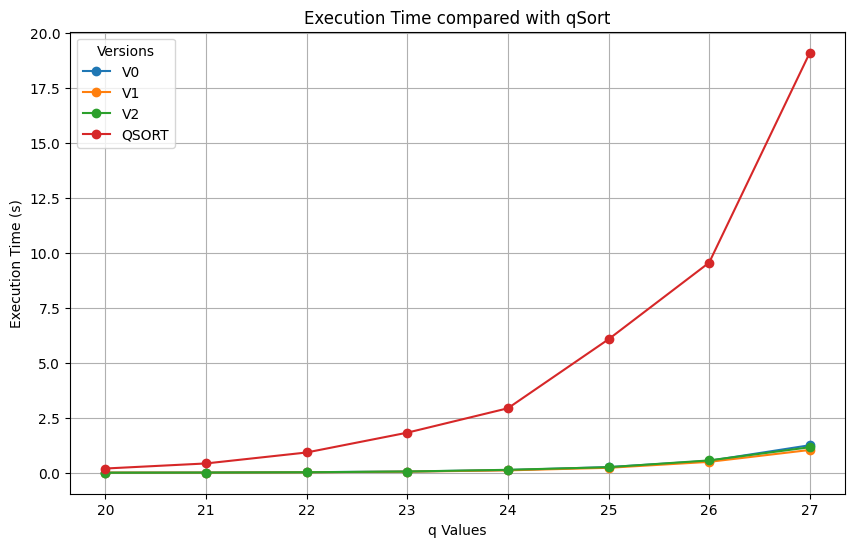
\includegraphics[width=1\linewidth]{assets/execution_time_qsort.png}
    \caption{Execution time compared with qSort}
    \label{fig:qSort}
\end{figure}

In Figure \ref{fig:versions} we focus on the execution times among the different versions. When the number of elements increases, we observe a significant improvement between the three versions.

\begin{figure}
    \centering
    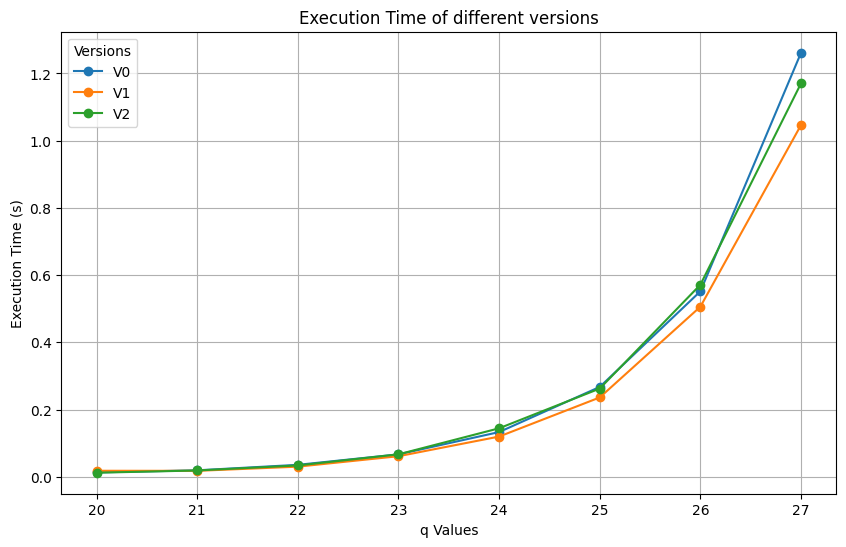
\includegraphics[width=1\linewidth]{assets/execution_time_versions.png}
    \caption{Execution times of different versions}
    \label{fig:versions}
\end{figure}

\subsection{Speedup}
Figure \ref{fig:speedup} shows the acceleration of each version in comparison with qSort.

\begin{figure}
    \centering
    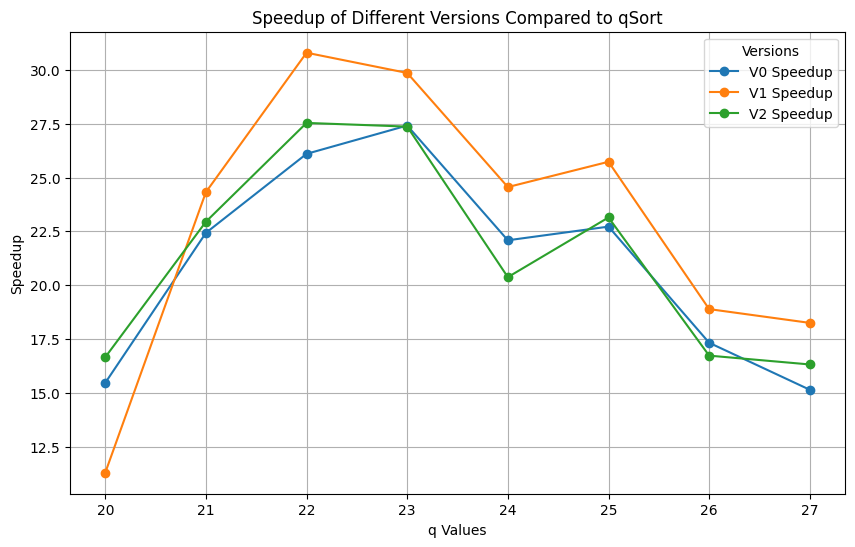
\includegraphics[width=1\linewidth]{assets/speedup.png}
    \caption{Speedup from qSort}
    \label{fig:speedup}
\end{figure}

\section{Conclusion}
In conclusion the implementation of Bitonic Sort with CUDA has a significant improvement in execution time and can be extremely effective, when handling large datasets.


\begin{thebibliography}{9}

\bibitem{sortvisualizer} \textit{Bitonic Sort Visualization}. Available \href{https://www.sortvisualizer.com/bitonicsort/}{here}.
\bibitem{shared memory} \textit{Shared Memory in CUDA}. Available 
\href{https://developer.nvidia.com/blog/using-shared-memory-cuda-cc/}{here}
\bibitem{CUDA picture} \textit{CUDA Memory Model}. Available \href{https://www.3dgep.com/cuda-memory-model/}{here}.
\end{thebibliography}

\end{document}
